\documentclass[12pt]{article}

\usepackage[slovene]{babel}
\usepackage[utf8]{inputenc}
\usepackage[T1]{fontenc}
\usepackage{amsmath}
\usepackage{bm}
\usepackage[a4paper, top=20mm]{geometry}
\usepackage{pdfpages}
\usepackage{listings}
\usepackage{url}
\usepackage{hyperref}
\lstset{
  basicstyle=\ttfamily\small, 
  language=Matlab,
  keywordstyle=\color{blue}
}

\begin{document}
\title{\textbf{Prepoznavanje uporabnika tipkovnice}}
\author{
  Leon Modic\\
  \and
  Matej Miočič\\
  \and
  Andraž Rozman\\
}
\maketitle

\section{Opis problema}
Različni ljudje razvijemo različne stile tipkanja. Naloga je, napišete program,
ki bo na podlagi količin, ki jih lahko izmerimo pri tipkanju (kot je časovni
zamik med posameznimi pari znakov), prepoznal uporabnika.

\section{Opis matematičnega modela}
Izbrali smo 47 tipk na tipkovnici in za vsakega uporabnika smo generirali več učnih
primerov matrik povprečnih časov velikosti $47 \times 47$
\[
  averageMatrix^{47 \times 47}=
  \begin{bmatrix}
    0.1301 & 0.0 & \dots & 0.0 & 0.0\\
    0.0 & 0.0 & \dots & 0.0 & 0.0\\
    \vdots & & & \vdots\\
    0.0 & 0.122 & \dots & 0.0 & 0.1\\
    0.0 & 0.0 & \dots & 0.735 & 0.0\\
  \end{bmatrix}
\]

Za vsakega izmed uporabnikov znotraj mape \texttt{data/} se generira $A_i$ matrika
(torej $A_{aljaz}$, $A_{andraz}$, $A_{leon}$, $A_{Matej}$), ki je sestavljena iz matrix povprečnih
časov za vsa merjenja določenega uporabnika.
\[
  A_i = \begin{bmatrix}
    p_1 & p_2 & \dots & p_m
  \end{bmatrix}
\]
Kjer so $p_i$ $2209 \times 1$ vektorji sestavljeni iz stolpcev matrike povprečnih časov ($averageMatrix$) zloženi
eden nad drugega. Nato naredimo SVD razcep:
$$A_i=U_iS_iV_i^T$$
$b$ je $2209 \times 1$ vektor sestavljen iz stolpcev matrike povprečnih časov, ki se je generirala za trenutno osebo, kateri želimo
določiti ime.
$$U_iS_iy_i = b \rightarrow y_i = (U_iS_i)^+b$$
$$min(||b-A_ix||) = min(||U_i^Tb-S_iy_i||)$$

\[
  names = \begin{bmatrix}
    "aljaz"\\
    "andraz"\\
    "leon"\\
    "Matej"
  \end{bmatrix},
  norms = \begin{bmatrix}
    1.92\\
    1.2\\
    1.44\\
    1.35
  \end{bmatrix}
\]
\section{Opis programske kode}
V našem projektu smo naredili dve funkciji za uporabnike: \textbf{\textit{main}} in \textit{saveMeasure}. 
S klicem funkcije \textit{main} uporabnik prične postopek ustvarjanja matrike, ki ga konča s pritiskom 
tipke \textit{escape}. Nato funkcija na podlagi ustvarjene matrike in drugih predhodno ustvarjenih matrik s 
\textit{saveMeasure}, prepozna uporabnika ali pa izpiše napako, če to ni mogoče. Ta proces deluje le, če je bilo 
ustvarjenih dovolj matrik s funkcijo \textit{saveMeasure}.

Funkcija \textbf{\textit{saveMeasure}} sprejme tri argumente. 
Prvi (\textit{user}) je tipa niz in označuje ime uporabnika, drugi (\textit{text}) je tipa niz in označuje naslov 
besedila, tretji (\textit{i}) pa je celoštevilskega tipa in predstavlja zaporedno številko matrike za dan naslov. 
Ob klicu funkcije z veljavnimi argumenti, se znotraj mape \textit{data} ustvari mapa z imenom uporabnika \textit{user} 
in znotraj te mape še mapa z imenom besedila \textit{text}, če katera od teh dveh map ne obstaja. 
Nato se kliče funkcija \textit{startMeasure} in prične se proces stvaritve matrike i. Ko \textit{startMeasure} 
vrne matriko, jo funkcija\textit{ saveMeasure} shrani v prej omenjeno mapo.

Funkcija \textbf{\textit{startMeasure}} ne sprejme nobenega argumenta.
Najprej ustvari tabelo veljavnih tipk, \textit{keys}.
To so črke angleške abecede, številke, ... Vse veljavne tipke so vidne na spodnji sliki (slika 1).
Ker je vseh veljavnih tipk 47, funkcija inicializira dve 47x47 matriki. 
Prva (\textit{times}) beleži vsoto časovnih razlik med pritiski dveh tipk, druga (\textit{n}) pa število teh pritiskov. 
Glavna while zanka funkcije se izvaja dokler ne pritisnemo tipke \textit{escape}. 
Na začetku vsake iteracije kličemo funkcijo \textit{KbQueueCheck}, ki vrne informacijo če je bil zaznan pritisk tipke, 
ter tabelo tipk, ki so bile pritisnjene. Funkcija \textit{KbQueueCheck} je del vmesnika \textit{PsychToolbox}, 
ki je potreben za izvajanje našega programa. Za delovanje funkcije \textit{KbQueueCheck} pa je sta potrebna klica 
funkcij \textit{KbQueueCreate} in \textit{KbQueueStart} še pred zanko. Nato s pomočjo funkcije \textit{find} 
preslikamo kodo tipke v indeks tipke znotraj tabele \textit{keys}. Če je preslikava trenutno pritisnjene tipke 
ter zadnje tipke veljavna, zabeležimo pritisk kombinacije teh dveh tipk in izračunamo ter prištejemo časovno 
razliko med tem in zadnjim pritiskom. Ko zaključimo while zanko izračunamo matriko povprečnih časov med dvema 
tipkama, timesAverage, ki jo funkcija tudi vrne, z naslednjim ukazom (ki tudi prepreči deljenje z 0): 
timesAverage = times./(n+(n==0))

\begin{figure}[h]
  \centering
  \label{slika1}
  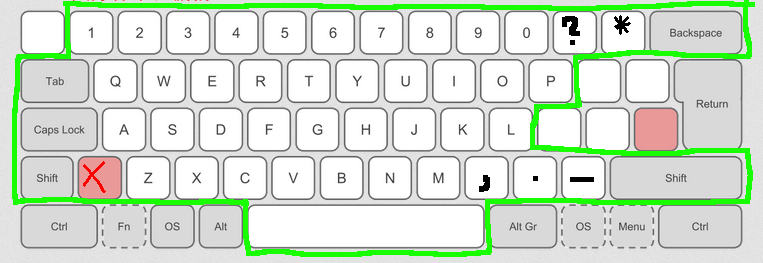
\includegraphics[scale=1.5]{keyboard}
  \caption{Veljavne tipke}
\end{figure}

\pagebreak
Struktura je razvidna v funkciji mainCalculate. Na začetku se premaknemo v mapo data, ki vsebuje mape z imeni oseb, 
ki so sodelovali pri projektu. To pomeni, da so pretipkali določen tekst in shranili matriko s funkcijo saveMeasure.\\
\newline
Nato se z zankami premikamo po mapah. S prvo zanko shranimo ime lastnika testov v spremenljivko userDirTemp z ukazom ls. 
Spremenljivko še transponiramo, da dobimo imena v vrsticah. Nato odstranimo presledke in imena dodamo v matriko 
names za kasnejšo uporabo.\\
\newline
Potem generiramo matriko A. Matrika je 2209 x m (kjer m predstavlja število testnih primerov), ki vsebuje meritve s 
povprečnimi časi med tipkami.\\
\newline
Kako jo naredimo? \\
\newline
Podobno kot prej se z zankami najprej premaknemo v mapo z imeni. Nato se premaknemo v mapo, ki vsebuje teste, 
glede na besedilo. Še z zadnjo zanko pa naložimo test (matriko 47x47) v spremenljivko X. X nato pretvorimo v vektor 
in dodamo k matriki A. \\
\newline
Ko dobimo matirko A za enega izmed tesnih oseb, naredimo SVD razcep in vstavljamo stvari v enačbo.

\section{Rezultati in komentarji rezultatov}
Uspešne rezultate smo dobivali že v začetku izdelave projekta. Najprej smo si izbrali besedilo dolgo 
približno 1000 znakov. Vsak izmed udeležencev ga je prepisal petkrat. Tako smo imeli shranjenih 15 testnih 
matrik. Ko smo testirali program na istem besedilu (pretipkali smo isto besedilo), nas je program prepoznal. 
Probali smo tudi na drugih besedilih, vendar smo dobili malo manj zanesljive odgovore. \\
\newline
Sklenili smo, da bomo dodali več testnih matrik, tokrat z različnimi besedili. Dodali smo še 8 različnih besedil, s povprečno 500 znaki vsak. Tokrat smo prepisali vsako besedilo samo enkrat. Dobili smo zelo pozitivne rezultate, saj nas je program zanesljivo prepoznal po treh stavkih. \\
\newline
Razumljivo pa je, da bo program ne bo vedel, kdo je uporabnik tipkovnice, če prepišemo prekratko besedilo, zato bo 
vračal različne odgovore, tudi če ga prepiše ista oseba:
\begin{figure}[h]
             \centering
             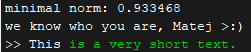
\includegraphics{correct_guy}
             \caption{Test1 programa z zelo kratkim besedilom.}
\end{figure}

\begin{figure}[h]
             \centering
             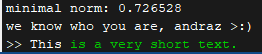
\includegraphics{wrong_guy}
             \caption{Test2 programa z zelo kratkim besedilom.}
\end{figure}

\section{Razdelitev dela v skupini}
Večinoma smo vso kodo pisali tako, da je tisti, ki je delil zalson dejansko tipkal,
skupaj pa smo razmišljali kaj na se napiše. 
\section{Reference in dejanksa koda}
\href{https://github.com/leonleon123/prepoznavanje_uporabnika_tipkovnice}{Github}
\end{document}
